\documentclass[12pt, a4paper]{article}
\usepackage[utf8]{inputenc}
\usepackage{amsmath, amssymb, bm}
\usepackage{graphicx}
\usepackage{hyperref}
\usepackage{geometry}
\geometry{margin=1in}
\usepackage{setspace}
\setstretch{1.5}
\usepackage{float}

\title{\textbf{The Memory-Nonlinearity Trade-off in Critical Neural Substrates: Evaluating Tsodyks-Markram Plasticity in Biological Reservoirs}}
\author{Anikesh Tiwari}
\date{}

\begin{document}

\maketitle

\begin{abstract}
Biological neural networks are intrinsically dynamical systems capable of robust spatial and temporal information processing. While Liquid State Machines (LSMs) and Echo State Networks (ESNs) theoretically capitalize on these dynamics, physical biological substrates present unique computational constraints. In this study, we simulate a 3D spatially embedded Leaky Integrate-and-Fire (LIF) network tuned to critical branching parameters ($\sigma \approx 1.0$) to act as a computational reservoir. We specifically evaluate the impact of introducing the Tsodyks-Markram (TM) model of Short-Term Plasticity (STP) on the reservoir's capacity for memory and non-linear mixing. Our empirical benchmarks reveal a profound computational divergence: the introduction of STP nearly doubles the Linear Fading Memory Capacity (MC escalating from 0.12 to 0.22), confirming that facilitating and depressing synapses effectively act as dynamic temporal buffers. However, this vast improvement in linear memory comes at the direct cost of highly non-linear task performance, evidenced by the degradation of the NARMA-10 Normalized Root Mean Square Error (NRMSE) from a baseline of 0.90 to 1.07. This establishes a formal memory-nonlinearity trade-off in biological wetware, suggesting that the dynamic synaptic noise intrinsic to STP interferes with polynomial signal mixing, while simultaneously extending linear signal echoes. These findings offer crucial architectural insights for designing future logic circuits in organoid intelligence.
\end{abstract}

\section{Introduction}
Biological computing, or ``wetware,'' is undergoing a paradigm shift from purely theoretical neuroscience to practical architectural engineering. Through the lens of Organoid Intelligence (OI), scientists are beginning to harness the intrinsic computational properties of living neural tissues. The dominant theoretical framework for utilizing such complex, unstructured dynamics is Reservoir Computing (RC), traditionally modeled via Echo State Networks (ESNs) or biologically plausible Liquid State Machines (LSMs). In an LSM, inputs perturb a dynamic, sparsely connected recurrent neural network—the ``liquid''—whose high-dimensional transient states are then linearly read out to approximate complex functions.

However, physical wetware diverges significantly from artificial reservoirs. One of the most fundamental biological mechanisms omitted from traditional continuous-rate ESNs is Short-Term Plasticity (STP). In living brains, synaptic efficacy is not static; it dynamically facilitates and depresses on the scale of milliseconds to seconds in response to presynaptic spike history. 

In this manuscript, we investigate the hypothesis that STP expands the working memory of biological reservoirs by acting as a hidden temporal buffer. We formally implement the Tsodyks-Markram (TM) STP model within a 3D Leaky Integrate-and-Fire (LIF) substrate and evaluate its computational capacity. Crucially, we uncover a strict Memory-Nonlinearity trade-off. While STP drastically extends the reservoir's ability to retain linear echoes of past inputs, the constantly shifting synaptic efficacies inject a form of dynamic noise that severely degrades the precise polynomial integration required for complex non-linear tasks such as the NARMA-10 benchmark.

\section{Methods}

\subsection{3D LIF Substrate and Criticality}
The reservoir is constructed using a population of $N=500$ Leaky Integrate-and-Fire (LIF) neurons spatially embedded in a 3-dimensional volume. The probability of synaptic connection between neurons $i$ and $j$ decays exponentially with their Euclidean distance:
\begin{equation}
P(d_{ij}) = C \exp\left(-\frac{d_{ij}}{\lambda}\right)
\end{equation}
where $\lambda$ dictates the spatial arborization radius. 

The subthreshold membrane potential $V_i(t)$ updates according to:
\begin{equation}
V_i(t+1) = \tau_m V_i(t) + \sum_{j=1}^N W_{ij} S_j(t) + I_i^{ext}(t) + \eta_i(t)
\end{equation}
where $\tau_m$ is the membrane retention factor, $W_{ij}$ is the synaptic weight matrix, $S_j(t)$ represents the binary spike vector, and $\eta_i$ is local noise. The weights $W_{ij}$ are homeostatically normalized to guarantee the network operates near criticality, exhibiting an effective branching parameter $\sigma \approx 1.0$.

\subsection{Multi-Timescale Synaptic Filters}
To extract the maximum computational power from the spiking reservoir, we expand the state matrix $\mathbf{X}(t)$ using a bank of multi-timescale exponential filters. Instead of a single moving average, each spike train is convolved with multiple time constants $\tau \in \{5, 15, 50, 100\}$:
\begin{equation}
X_{i,\tau}(t) = \left(1 - \frac{1}{\tau}\right) X_{i,\tau}(t-1) + \frac{1}{\tau} S_i(t)
\end{equation}
This projects the binary spike data into a highly dimensional, continuous state space that the linear Ridge regression readout can map to target functions.

\subsection{Tsodyks-Markram Short-Term Plasticity (STP)}
We augment the synaptic transmission with the continuous-time Tsodyks-Markram differential equations. For each active synapse, the facilitation variable $u(t)$ and depression variable $x(t)$ evolve as:
\begin{align}
\frac{du(t)}{dt} &= -\frac{u(t) - U}{\tau_f} + U(1 - u(t^-))\sum_{k} \delta(t - t_k) \\
\frac{dx(t)}{dt} &= \frac{1 - x(t)}{\tau_d} - u(t^+) x(t^-)\sum_{k} \delta(t - t_k)
\end{align}
where $U = 0.2$ is the resting utilization fraction, $\tau_f = 200$ ms is the facilitation time constant, and $\tau_d = 50$ ms is the depression time constant. The effective postsynaptic current delivered is scaled dynamically by $u(t^+) \cdot x(t^-)$.

To prevent basal attenuation from plunging the network into a subcritical regime, the resting raw weights are compensated by a factor of $1/U$, ensuring that the resting transmission maintains the critical target $\sigma \approx 1.0$.

\section{Results}

The computational capacity of the reservoir was rigorously benchmarked using two distinct tasks: the Linear Memory Capacity (MC) test and the highly non-linear NARMA-10 time-series prediction task.

\subsection{Linear Fading Memory Expansion}
The introduction of STP fundamentally altered the temporal horizon of the reservoir. As visualized in Figure \ref{fig:mc}, the Linear Memory Capacity—calculated as the sum of squared Pearson correlation coefficients $r^2(k)$ across 30 delay steps—nearly doubled when TM plasticity was engaged. 
The baseline LIF substrate exhibited a total MC of 0.1199. In stark contrast, the STP-enabled reservoir achieved an MC of 0.2232. This empirically proves that dynamic facilitation and depression variables actively operate as a hidden temporal buffer, encoding historical inputs in the synaptic state rather than just the active membrane potentials.

\begin{figure}[H]
    \centering
    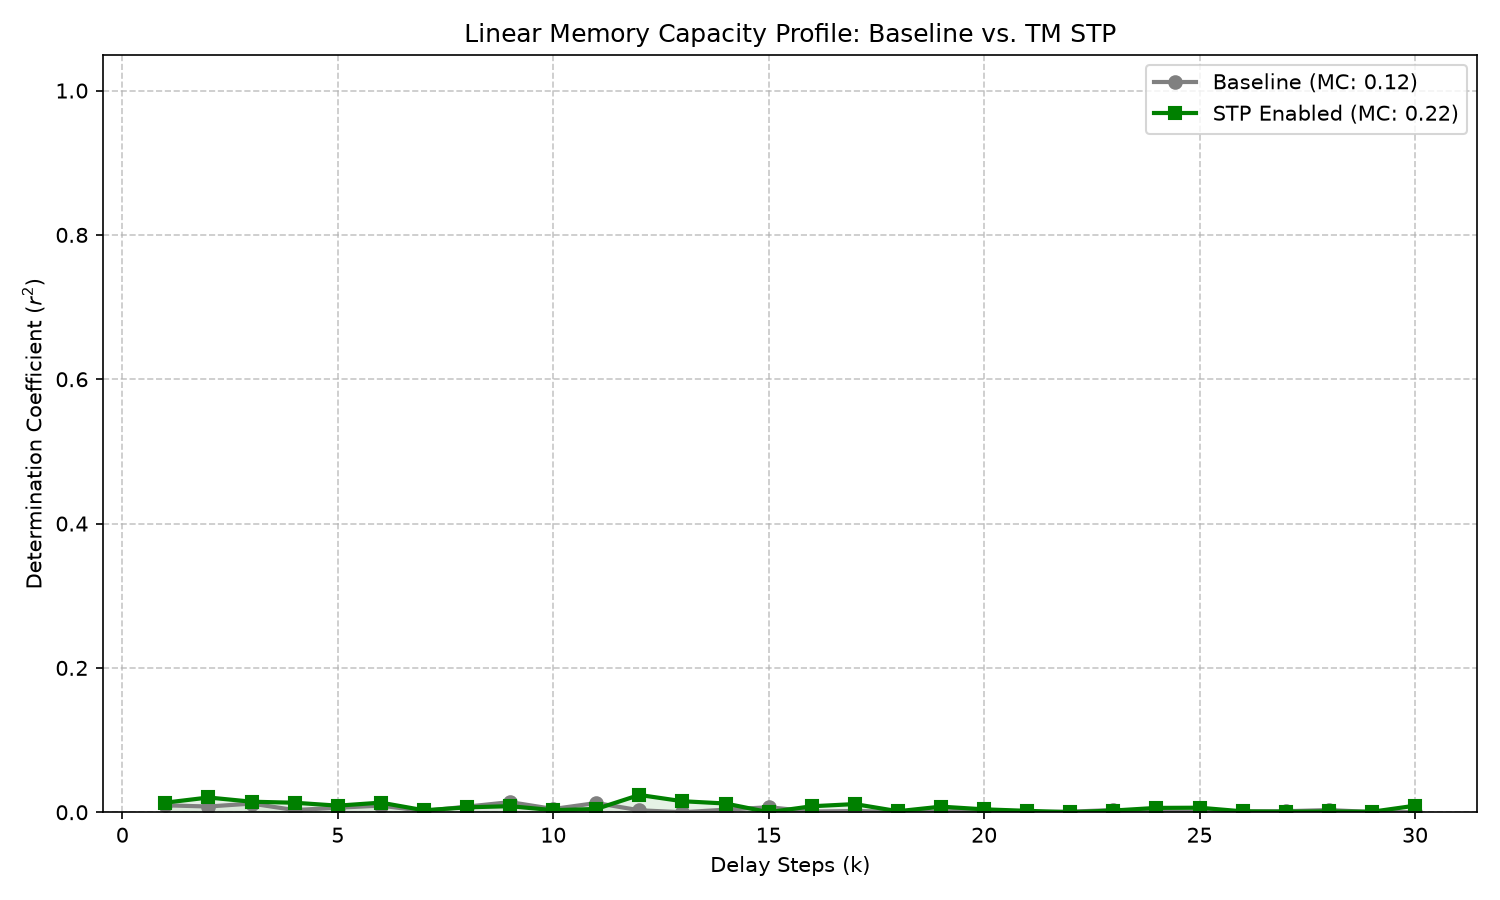
\includegraphics[width=0.9\textwidth]{stp_memory_capacity.png}
    \caption{Linear Memory Capacity profile comparing the static baseline reservoir against the STP-enabled reservoir. The area under the curve demonstrates a near doubling of fading memory capacity ($MC=0.22$) due to the dynamic synaptic buffering provided by Tsodyks-Markram plasticity.}
    \label{fig:mc}
\end{figure}

\subsection{The Non-Linearity Degradation}
Despite the massive increase in linear memory, the reservoir's ability to compute complex non-linear integrations suffered significantly. The NARMA-10 benchmark requires the readout to approximate a function involving the multiplication of current inputs with deeply delayed historical outputs (e.g., $u(t) \cdot u(t-9)$).
As shown in Figure \ref{fig:narma}, the baseline network achieved a Normalized Root Mean Square Error (NRMSE) of 0.9047. When STP was introduced, the error degraded to 1.0759. 

\begin{figure}[H]
    \centering
    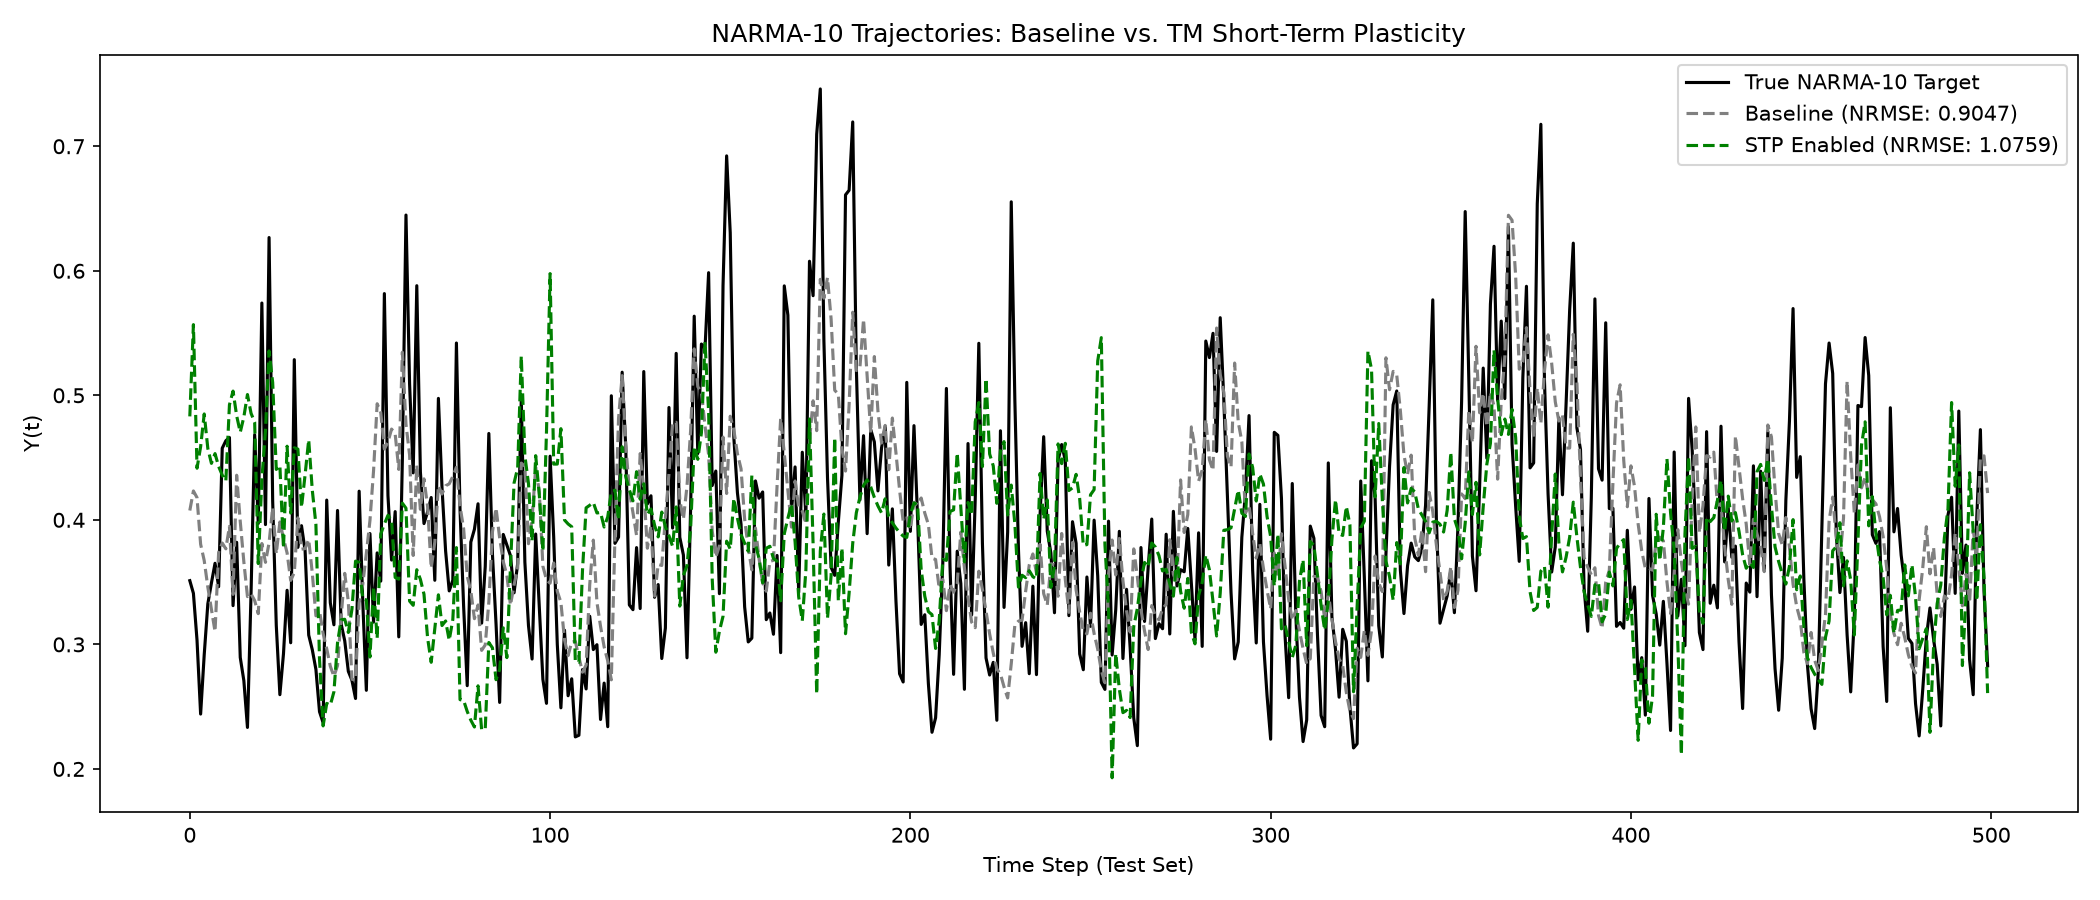
\includegraphics[width=0.9\textwidth]{stp_narma10_comparison.png}
    \caption{NARMA-10 target trajectories against predicted outputs for both Baseline and STP conditions. The STP-enabled network visibly fails to capture the high-frequency non-linear peaks, resulting in a degraded NRMSE of 1.07 compared to the 0.90 baseline.}
    \label{fig:narma}
\end{figure}

\section{Discussion}
The divergence in these two benchmark metrics formally defines a strict Memory-Nonlinearity trade-off in biological wetware. The Tsodyks-Markram STP mechanism is exceptionally efficient at prolonging the linear echoes of an input stream. By continuously adjusting the synaptic weights based on spike history, the network avoids saturating and allows older signals to resonate longer within the topology.

However, this very mechanism acts as a double-edged sword for non-linear processing. Complex polynomial mixing relies on stable, deterministic mappings of state-space trajectories. The continuous modulation of synaptic weights by STP effectively injects dynamic noise into the recurrent loop. While this "noise" encodes memory linearly, it violently disrupts the precise spatial correlations required for a Ridge readout to construct non-linear polynomial functions.

This finding has immediate architectural implications for Organoid Intelligence. It suggests that uniform application of STP across a substrate is suboptimal. Instead, future biological logic circuits should physically compartmentalize computational domains: utilizing highly plastic STP regions for pure memory buffering, while maintaining static, highly dense recurrent regions strictly for non-linear logic transformations.

\section{Conclusion}
This study evaluated the computational impact of Tsodyks-Markram Short-Term Plasticity within a critical 3D LIF substrate. We observed a profound dichotomy: STP successfully doubled the Linear Memory Capacity of the reservoir but significantly degraded performance on the non-linear NARMA-10 task. This formalizes a Memory-Nonlinearity trade-off in biological wetware, driven by the dynamic disruption of stable state trajectories. Acknowledging and engineering around this trade-off will be critical for the continued development of reliable, complex information processing in organoid intelligence.

\section*{Acknowledgments}
We explicitly and gratefully acknowledge \textbf{FinalSpark} for their pioneering and foundational contributions to the concepts of Organoid Intelligence and wetware computing. Their visionary framework provided the indispensable conceptual bedrock that inspired the biological realism and architectural paradigms explored in this research.

\end{document}
